\chapter{研究結果}

\section{感測器檢測狀況}
(圖片)\\
使用的三個感測器皆已成功完成線路連接,且能及時讀取氣體濃度,但唯獨 MH-Z19B 重新啟動時需等待其熱機完畢方可使用。

\section{模型準確度}
\begin{itemize}
	\item 決策樹\\
	\begin{figure}[H]
		\centering
		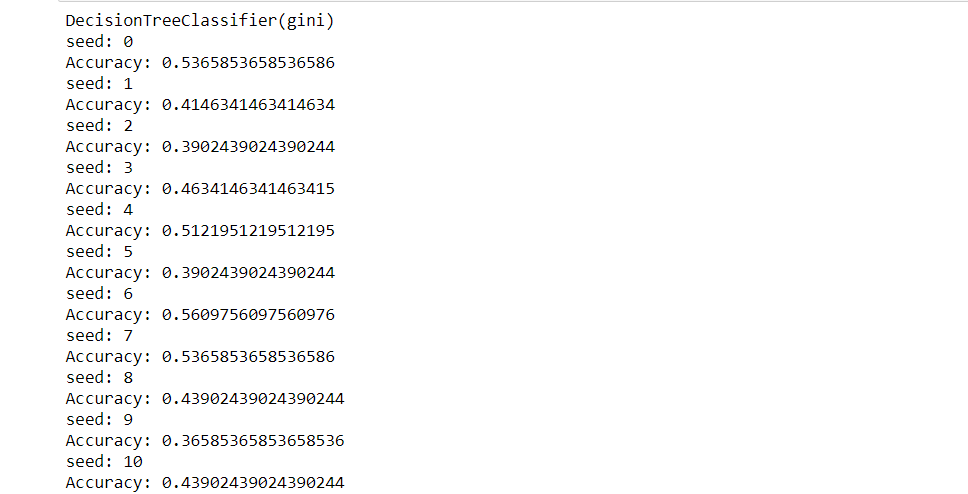
\includegraphics[width=0.8\textwidth]{pic/decisiontree.png}
	\end{figure}
	\item KNN\\
	\begin{figure}[H]
		\centering
		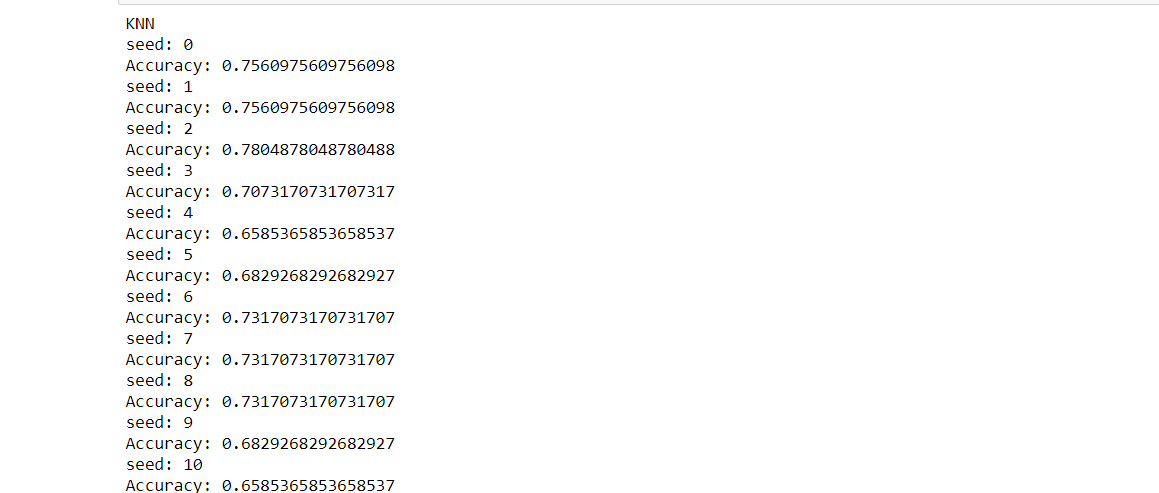
\includegraphics[width=0.8\textwidth]{pic/knn.png}
	\end{figure}
	\item 單純貝氏\\
	\begin{figure}[H]
		\centering
		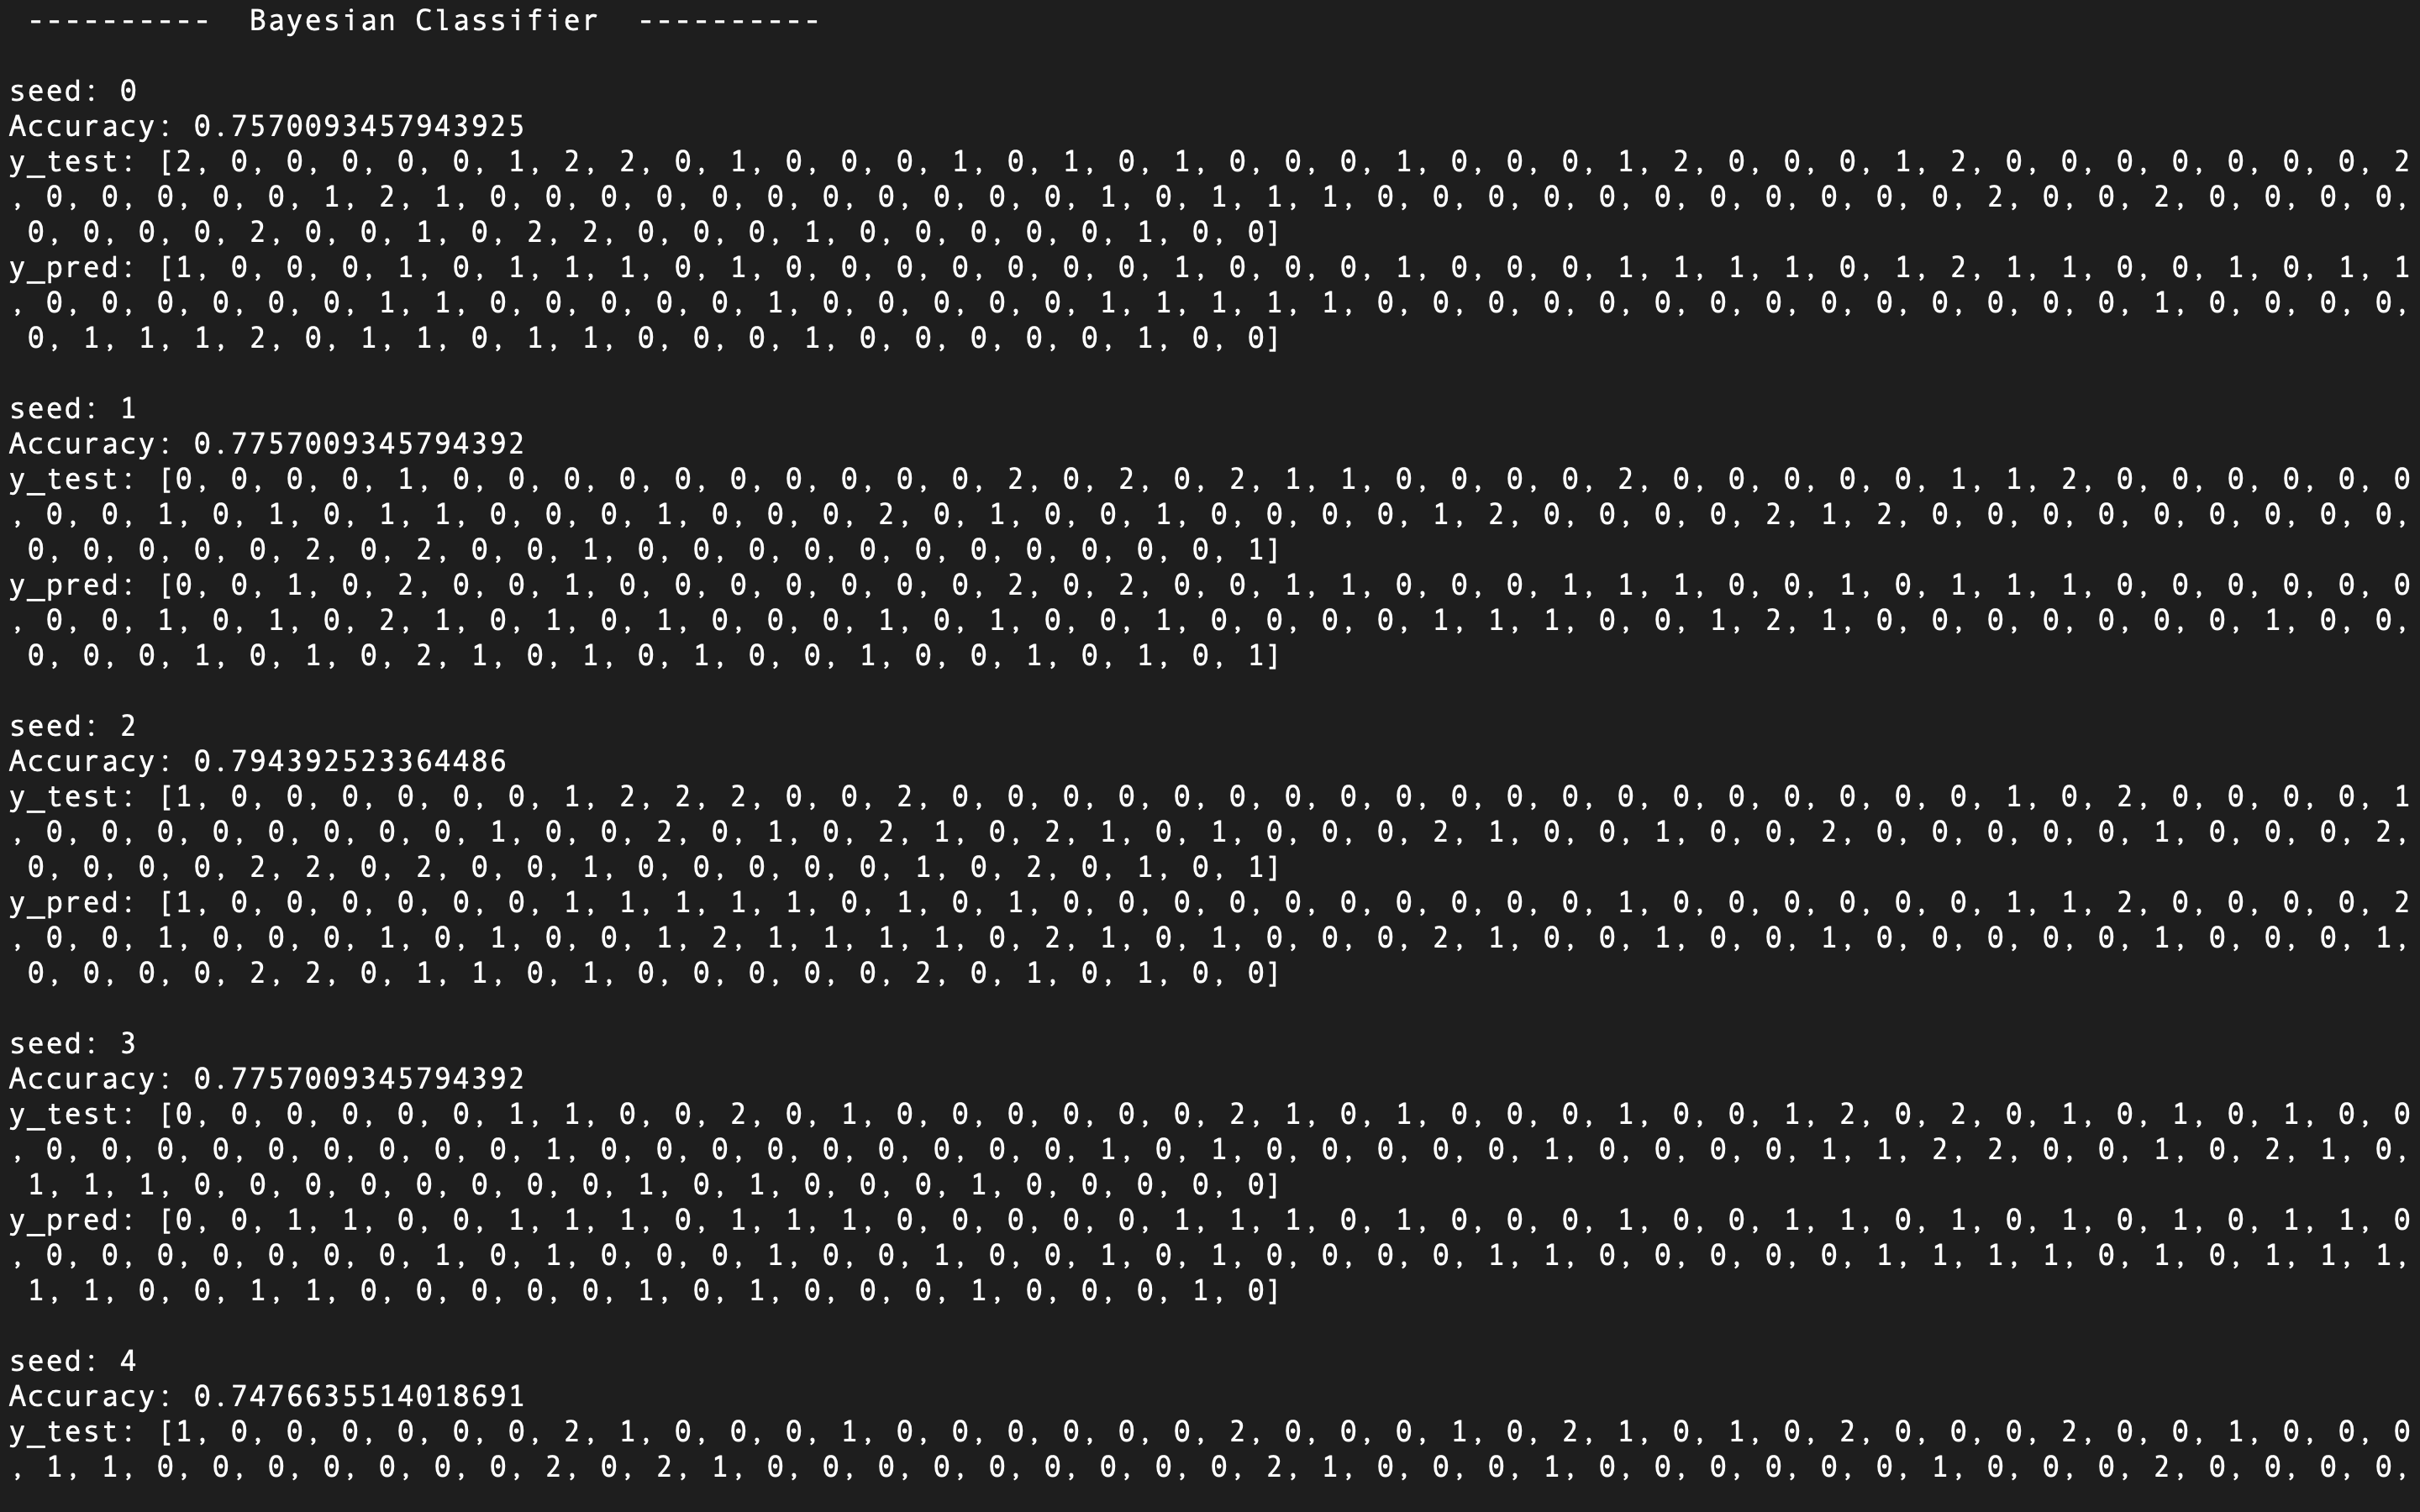
\includegraphics[width=0.8\textwidth]{pic/Bayesian.png}
	\end{figure}
	\item AdaBoost\\
	\begin{figure}[H]
		\centering
		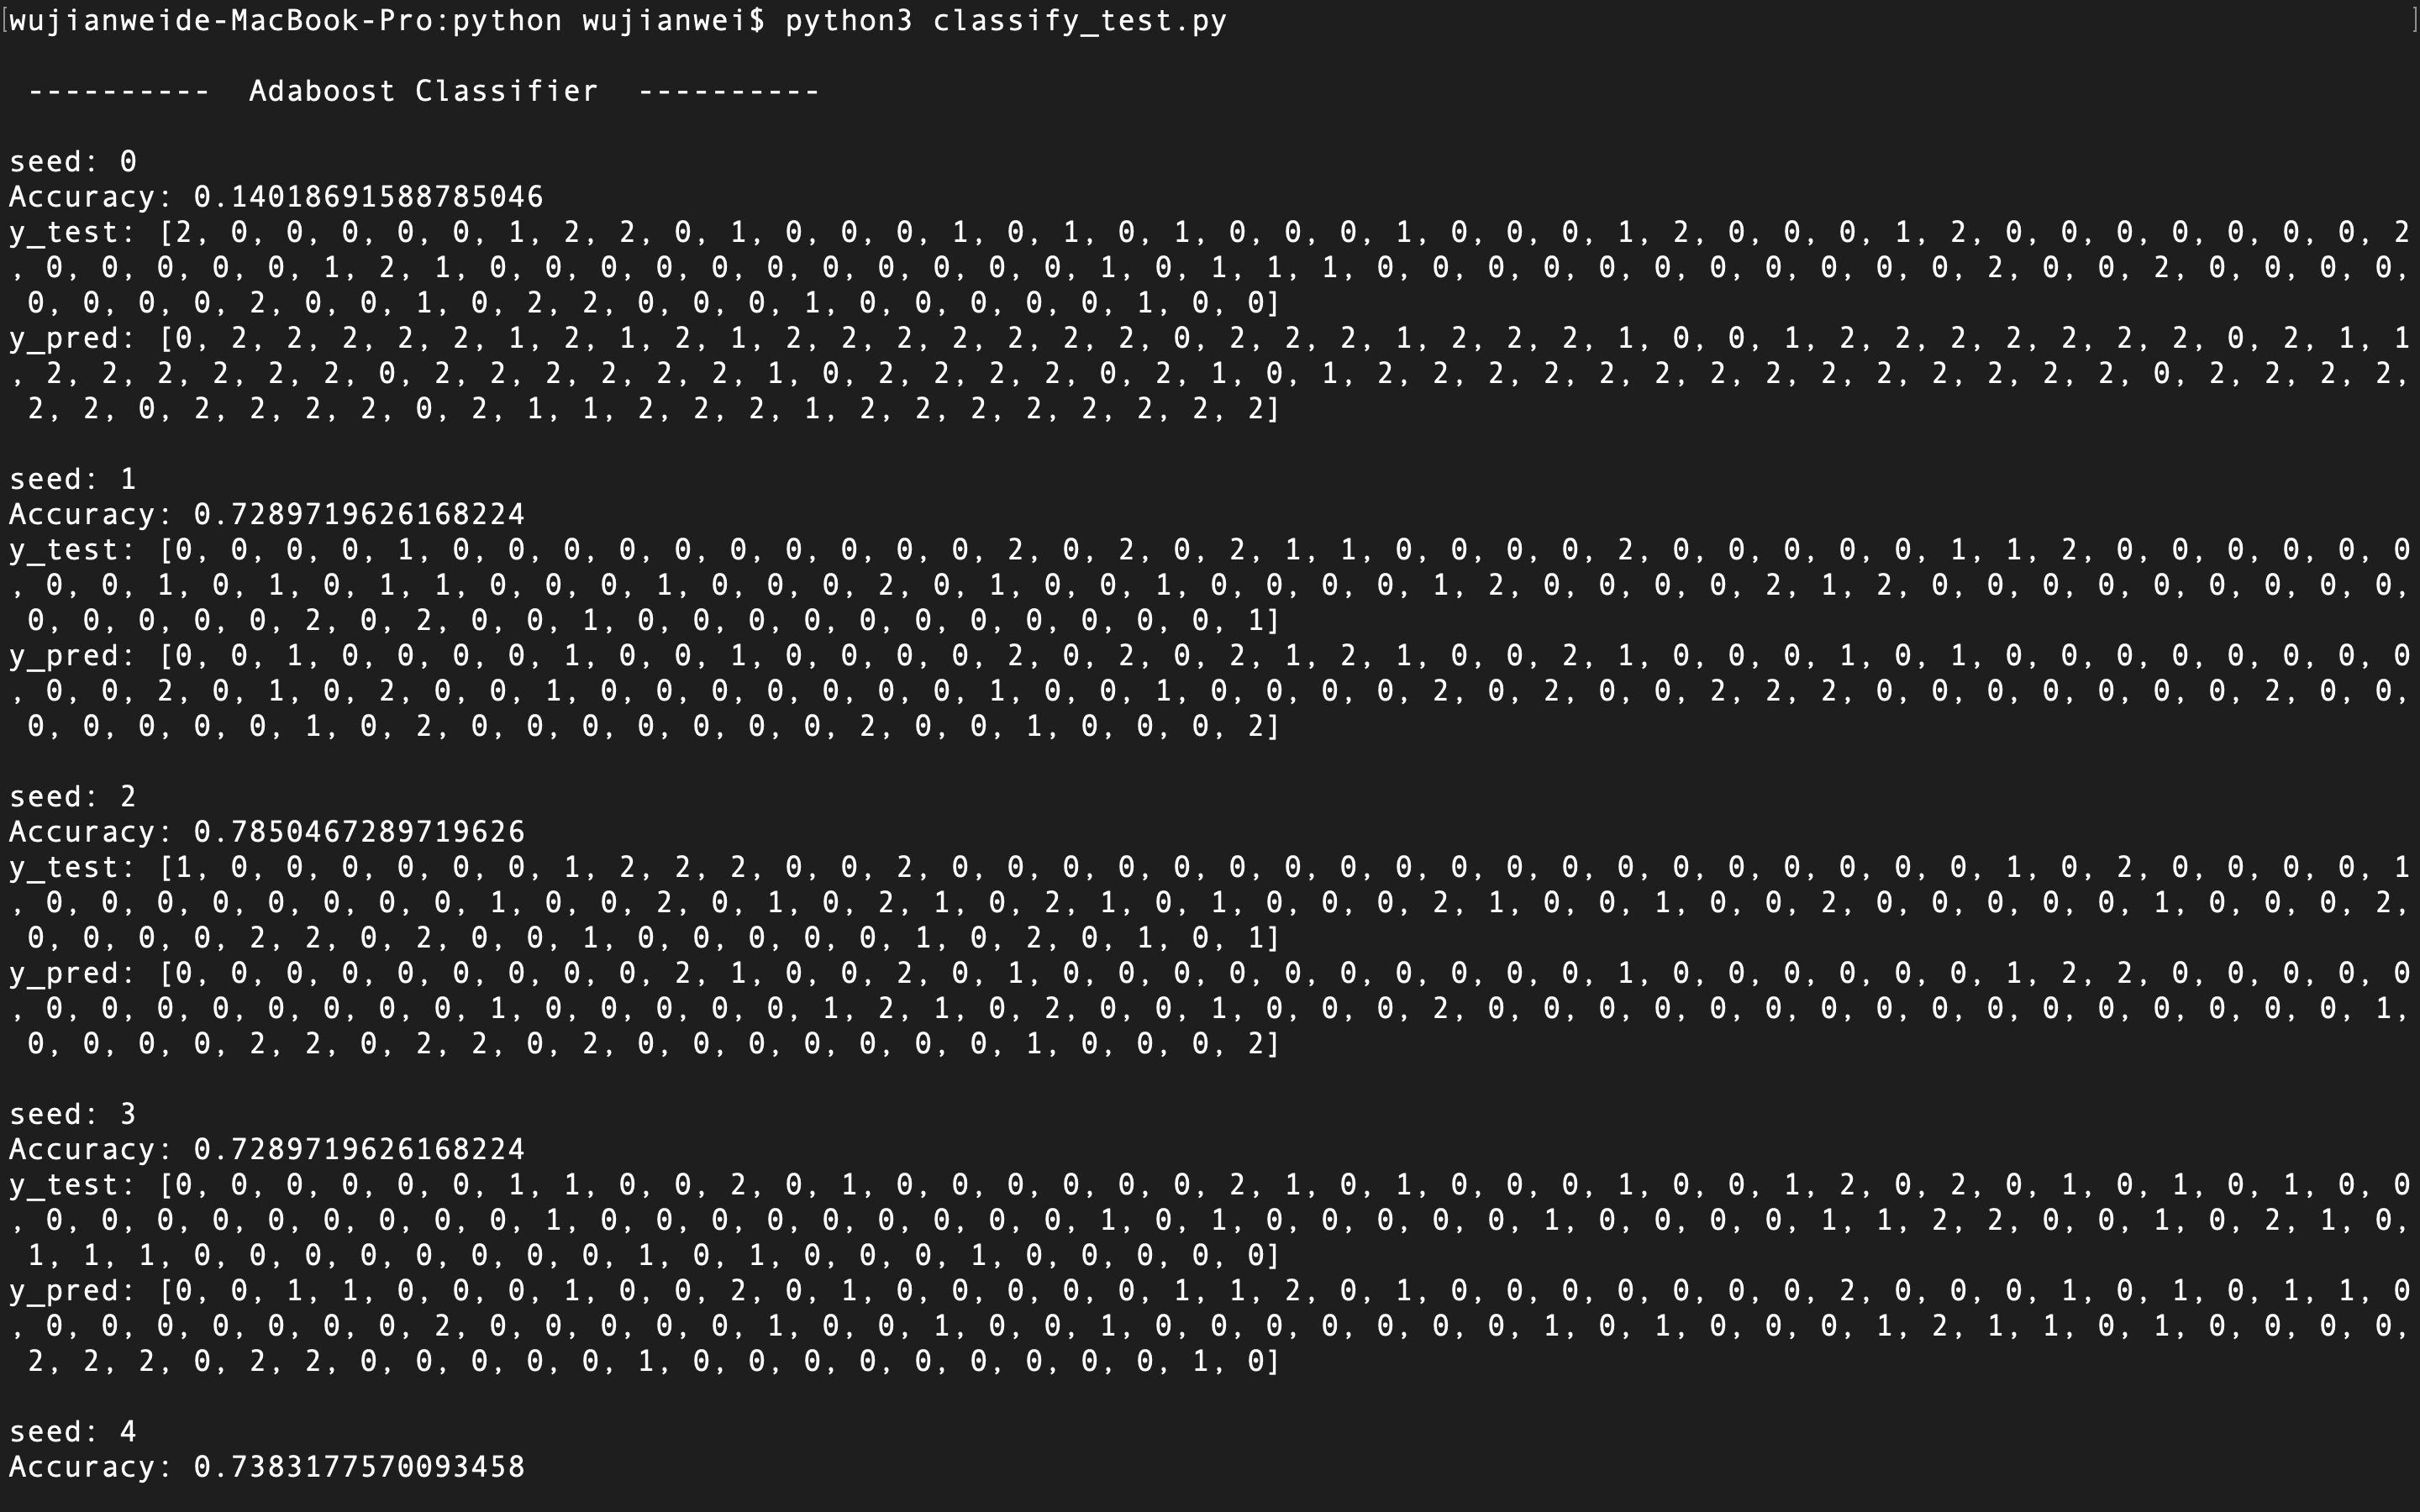
\includegraphics[width=0.8\textwidth]{pic/Adaboost.png}
	\end{figure}
\end{itemize}

\section{設備外型}
\begin{figure}[H]
	\centering
	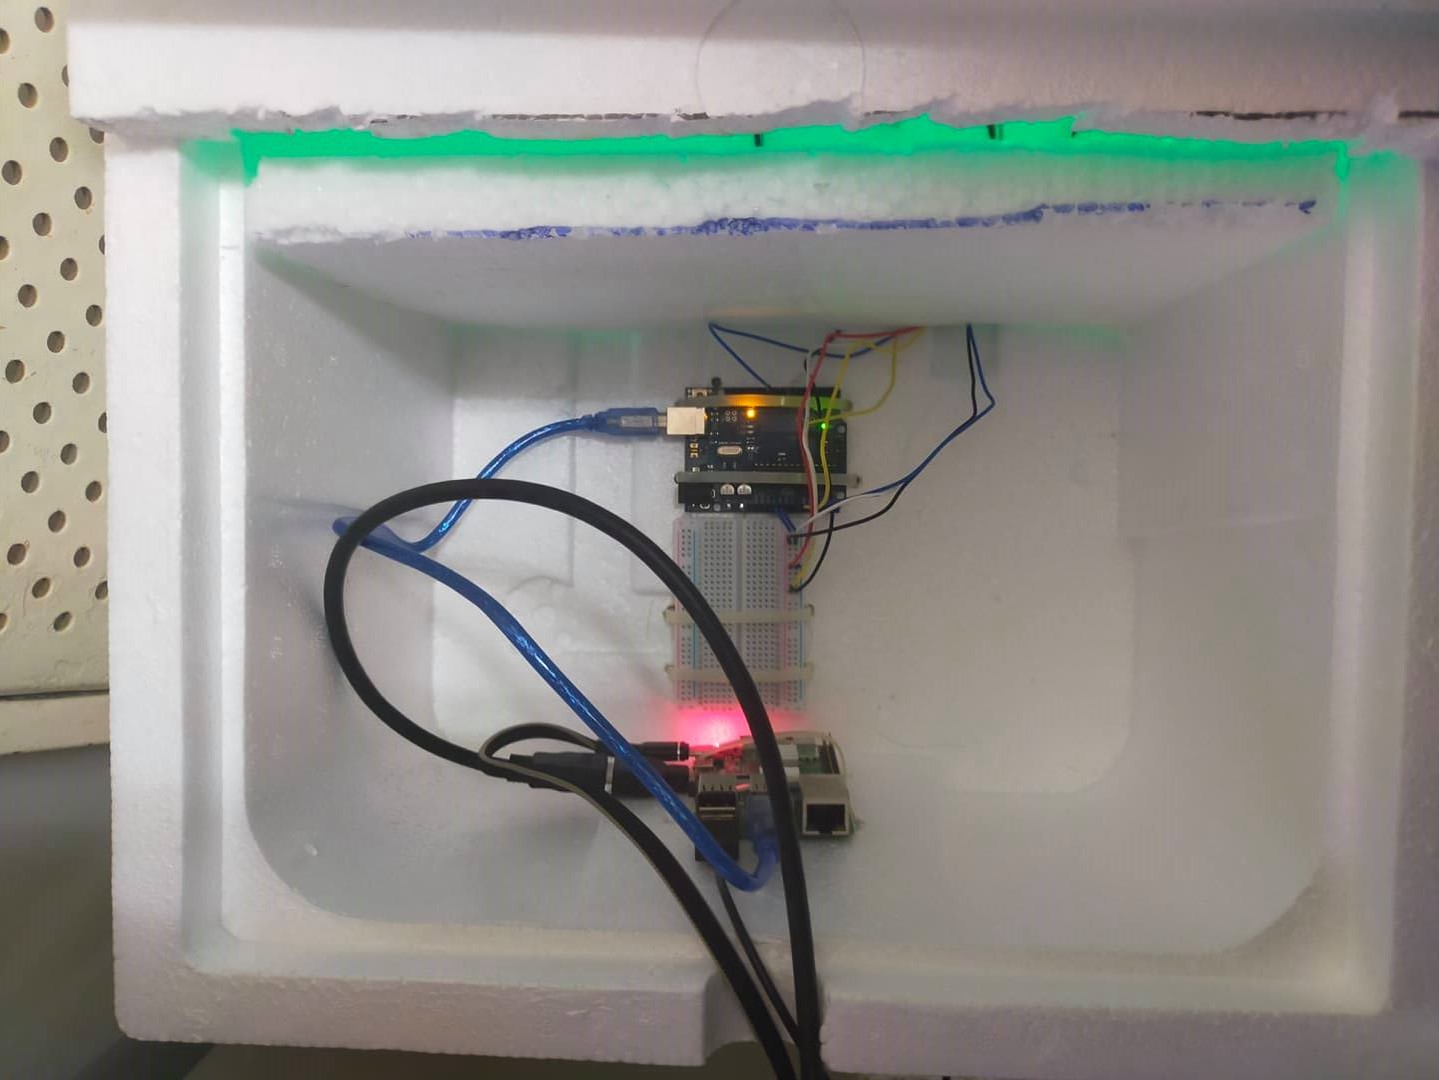
\includegraphics[width=0.5\textwidth]{pic/box(1).jpg}
\end{figure}
\begin{figure}[H]
	\centering
	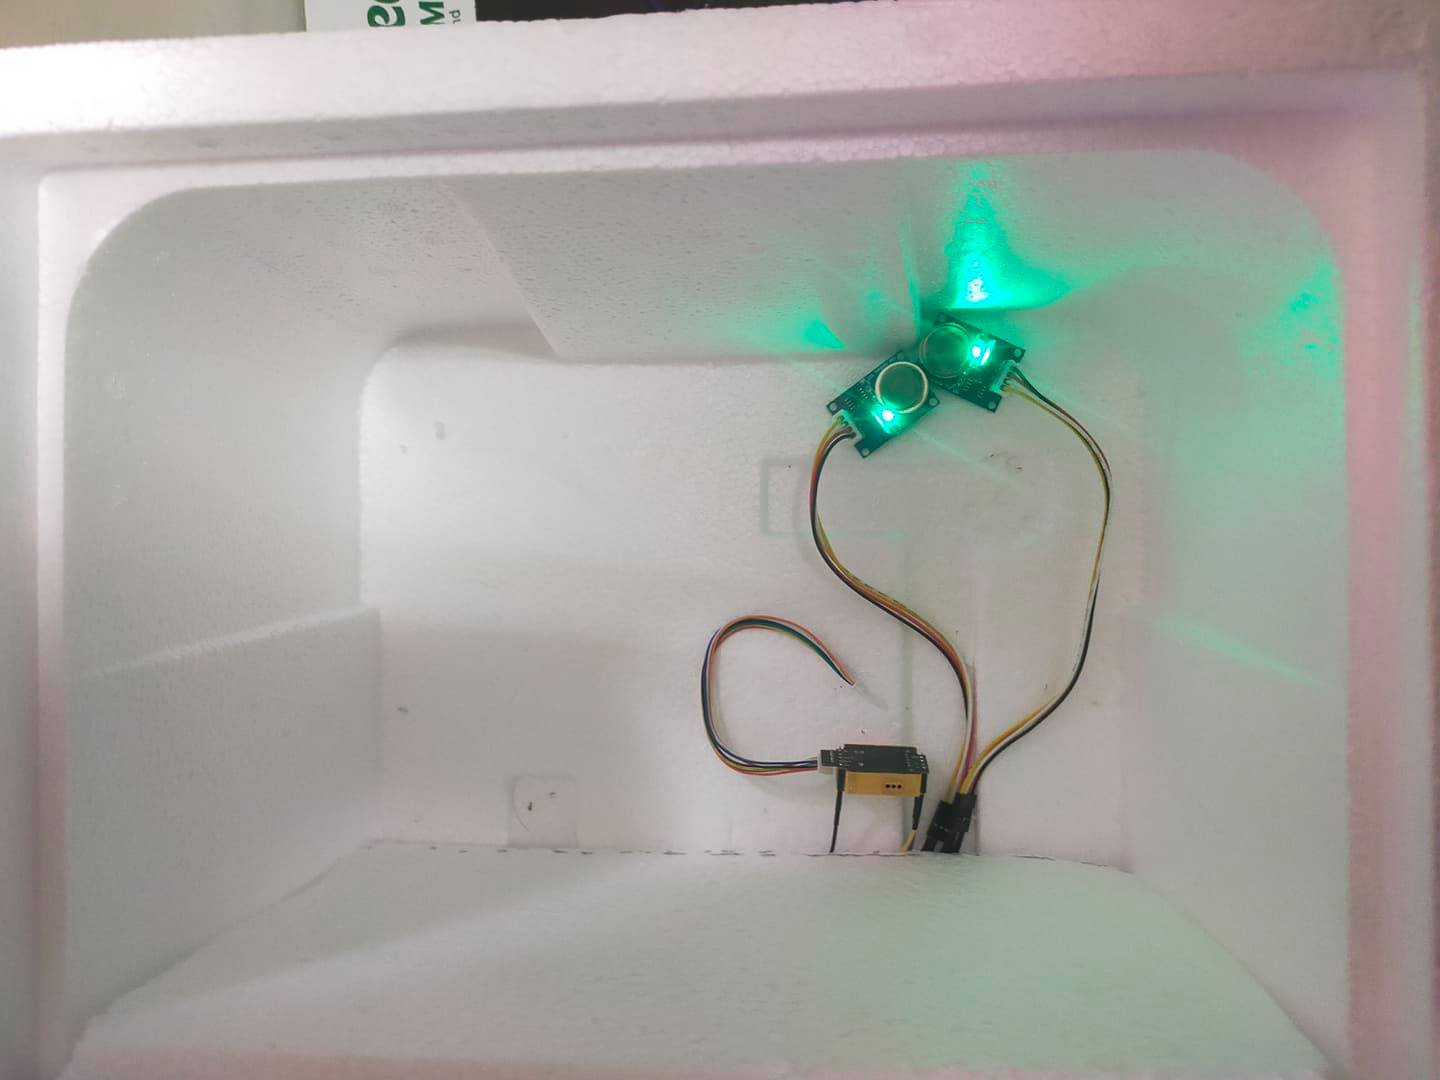
\includegraphics[width=0.5\textwidth]{pic/box(2).jpg}
\end{figure}
\begin{figure}[H]
	\centering
	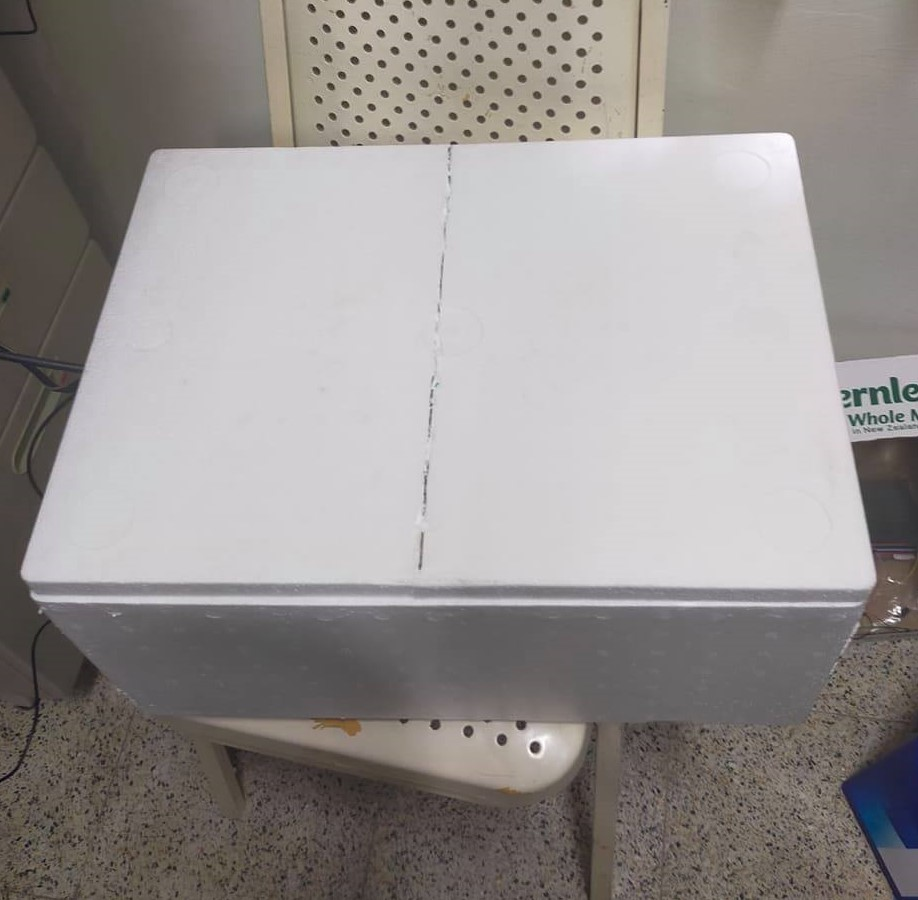
\includegraphics[width=0.5\textwidth]{pic/box(3).jpg}
\end{figure}